\documentclass[10pt,a4paper]{article}
\usepackage[utf8]{inputenc}
\usepackage[english]{babel}
\usepackage[T1]{fontenc}
\usepackage{amsmath}
\usepackage{amsfonts}
\usepackage{amssymb}
\usepackage{subcaption}
\usepackage{makeidx}
\usepackage{graphicx}
\usepackage{fourier}
\usepackage{listings}
\usepackage{color}
\usepackage{hyperref}
\usepackage[left=2cm,right=2cm,top=2cm,bottom=2cm]{geometry}
\author{Tommy Müller, Marcus Dittrich, Vincent Noculak}
\title{Quadrupol-Massenfilter}


\begin{document}



\section{Theoretische Vorbereitung}

\subsection{Quadrupolfeld}

Das elektrische Potential einer Ladungsverteilung aus Punktladungen ist

\begin{equation}
	\phi(\textbf{r}) = \frac{1}{4 \pi \epsilon_0 \sum_{j} \frac{q_j}{|\textbf{r}-\textbf{r}_j|}}
\end{equation}

Es kann genähert werden durch

\begin{equation}
	\phi(\textbf{r}) = \frac{1}{4 \pi \epsilon_0} \sum_{j} q_j (\frac{1}{r} + \frac{\textbf{r} \textbf{r}_j}{r^3} + \frac{3(\textbf{r}\textbf{r}_j)^2 - \textbf{r}^2 \textbf{r}^2_j}{r^5})
\end{equation}

Hier ist der erste Term der Coulomb-, der zweite der Dipol- und der dritte der Quadrupolbeitrag. Wenn die Gesamtladung und das Dipolmoment im System verschwinden, so bleibt nur der Quadrupolbeitrag übrig. Das Potential kann dann geschrieben werden als

\begin{equation}
	\phi(\textbf{r}) =  - \frac{1}{2} \phi _0 (\lambda x^2 + \sigma y^2 + \gamma z^2)
	\label{potential1}
\end{equation}

mit

\begin{align}
	\lambda = 2 Q{xx} -Q{yy}-Q{zz}\\
	\sigma = 2 Q{yy}-Q{xx}-Q{zz}\\
	\gamma = 2 Q{zz}-Q{xx}-Q{yy}\\
	Q{xx} = \frac{1}{3} \sum_{j} q_j (3 x_j^2 - r_j^2)
\end{align}

Aus der Laplace-Gleichung($\Delta \phi = 0$) folgt aus \ref{potential1}

\begin{equation}
	\lambda + \sigma + \gamma = 0
\end{equation}

Diese Gleichung lässt sich mit $\lambda = - \sigma = \frac{1}{r_0^2}$ und $\gamma = 0$ lösen. Mit dieser Lösung erhalten wir das Potential

\begin{equation}
	\phi (\textbf{r}) = - \frac{1}{2} \phi _0 \frac{(x^2 - y^2)}{r_0^2}
	\label{potential2}
\end{equation}

Die Äquipotentialflächen für dieses Potentials sind Hyperbeln. Elektroden, die der Form der Äquipotentialflächen haben, entsprechen denen eines Quadrupolmassenfilters. Legt man bei an den Elektroden, die dieses Potentialfeld erzeugen, eine mit Gleichspannung überlagerte Wechselspannung an($\phi _0 = U + V cos(\omega t)$), so erhält man für die Bewegungsgleichung eines Ions in diesem Feld die Differentialgleichungen

\begin{align}
	m\frac{d^2x}{dt^2} + Q(U + V cos(\omega t)) \cdot \frac{x}{r_0^2} = 0 
	\label{xdgl1}\\
	m\frac{d^2y}{dt^2} - Q(U + V cos(\omega t)) \cdot \frac{y}{r_0^2} = 0 
	\label{ydgl1}\\
	m\frac{d^2z}{dt^2} = 0 \\
\end{align}

Aus den Gleichungen kann gelesen werden, dass es in x-Richtung eine rücktreibende Kraft zum Koordinatenursprung gibt, während die Kraft in y-Richtung defokussierend ist.

Substituiert man $\omega t = 2\epsilon$, $a = \frac{8 e U}{m r_0^2 \omega^2}$ und $q = \frac{4 e V}{m r_0^2 \omega^2}$, so erhält man durch einsetzen in \ref{xdgl1} und \ref{ydgl1} folgende Gleichungen.

\begin{align}
	\frac{d^2x}{dt^2} + (a + 2q \cdot cos(2\epsilon)) x = 0\\
	\frac{d^2y}{dt^2} - (a + 2q \cdot cos(2\epsilon)) y = 0
\end{align}

Dies sind Mathieusche Differentialgleichungen.



\subsection{Mathieusche Differentialgleichung und Stabilitätsdiagramme}

Mathieusche Differentialgleichung sind Differentialgleichungen folgender Form:

\begin{equation}
	\frac{d^2u(x)}{dx^2} + (a + 2q \cdot cos(2x)) u = 0
\end{equation}

Auf die Gleichung gibt es stabile(beschränkte) und instabile(nicht beschränkte) Lösungen. Ob es eine stabile Lösung gibt ist von $a$ und $q$ abhängig. Trägt man die Bereiche für a und q, die stabile Lösungen liefern, in ein Diagramm ein, so erhält man ein sogenanntes Stabilitätsdiagramm. In Abbildung \ref{stabilitatsdiagramm1} kann ein Stabilitätsdiagramm für den Quadrupol-Massenfilter gesehen werden. Der stabile Bereich hat grob die Form eines Dreiecks. Wegen $\frac{a}{q} = \frac{8 U}{4 V} = \frac{2 U}{V}$ liegen alle Ionen bei festen Spannungen auf einer Geraden. Eine solche Gerade ist exemplarisch in der Abbildung zu sehen. 

Ändert man das Verhältnis $\frac{U}{V}$, so verändert man auch die Steigung der Gerade, auf der die Ionen liegen. Folglich kann man durch das Einstellen von $\frac{U}{V}$ das Intervall stabiler q-Werte bestimmen. Weil q direkt antiproportional zur Masse eines Ions zusammenhängt, lässt sich mit dem eingestellten Wert für $\frac{U}{V}$ auch das stabile Massenintervall für Ionen einstellen. Das macht man sich im Quadrupol-Massenspektrometer zunutze, um Ionen mit bestimmten Massen herauszufiltern.

\begin{figure}[h]
	\centering
	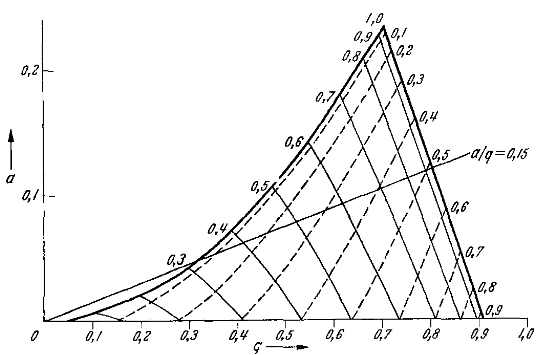
\includegraphics[scale = 0.8]{stabilitatsdiagramm.png}
	\caption{Stabilitätsdiagramm eines Quadropol-Massenfilters}
	\label{stabilitatsdiagramm1}
\end{figure}

\subsection{Quadrupol-Massenspektrometer}

In dieser Art von Massenspektrometer werden Ionen mithilfe eines elektrischen Quadrupolfelds gefiltert. Das verwendete Quadrupolfeld entspricht dem in \eqref{potential2} und wird durch vier in z-Richtung parallel liegende Stabelektroden realisiert. Mithilfe der Stabilitätsdiagramme, die sich aus dem Lösen der Bewegungsgleichung des elektrischen Feldes ergeben, kann man zeigen, dass nur Ionen mit spezifischen Ladungen, die in bestimmten Bereichen liegen, entlang der z-Achse durch den Massenfilter gelangen können. Andere Ionen werden abgelenkt und treffen auf die Elektroden.

\subsection{Ionisierungspotential}

Das Ionisierungspotential beschreibt die Energie, die aufgewendet werden muss, um ein Molekül zu ionisieren. Die Ionisierung kann zum Beispiel dadurch verursacht werden, dass Elektronen, die durch ein elektrisches Feld beschleunigt wurden, mit einer gewissen kinetischen Energie auf ein Molekülgas treffen.

Übersteigt die Energie der Elektronen die Ionisierungsenergie des Moleküls, so kann es zusätzlich zur Ionisation in kleinere Moleküle oder atomare Bestandteile zerfallen. Haben die Zerfallsprodukte eine Gesamtladung, so erscheinen ihre Massen, wenn sie durch ein Massenspektrometer laufen, als Peaks. 


\end{document}